\chapter{Residuos y polos}

\section{Singularidades y residuos}

Recordemos que un punto $z_0$ es una \textit{punto singular} de $f$, si ésta no es analítica en $z_0$ pero es analítica en algún punto de cada vecindad de $z_0$. Por ejemplo, tenemos que 0 es un punto singular de $1/z$ y, también, de $Log(z)$. De hecho, en esta última función, cada punto del semieje real negativo es un punto singular de $Log(z)$.

\begin{defi}
Un punto $z_0$ se dice \textbf{singular aislado} de $f$ si existe una vecindad de $z_0$ donde $f$ es analítica excepto en $z_0$.
\end{defi}

\begin{ejemplo}
El 0 es un punto aislado de $1/z$, pero no es punto aislado de $Log(z)$, pues toda vecindad centrada en el origen contiene puntos del semieje real negativo, en los que $Log(z)$ no es analítica.
\end{ejemplo}

\begin{ejemplo}
La función
$$\frac{z+1}{z^3(z^2+1)}$$

tiene tres puntos singulares aislados: $z = 0, \pm i$.
\end{ejemplo}

\begin{ejemplo}
La función 
$$\frac{1}{\sin(\pi z)}$$

tiene como puntos singulares aislados los $z = n \in \mathbb{Z}$.

En cambio, la función
$$\frac{1}{\sin\left( \frac{\pi}{z} \right)}$$

tiene los puntos singulares $z = 0$ y $z = 1/n$, con $n = \pm 1, \pm 2, \dots$, situados todos en el segmento del eje real entre $z = -1$ y $z = 1$. Cada punto singular, salvo $z = 0$, es aislado. El punto singular $z = 0$ no es aislado porque para toda vecindad centrada en el origen, existe $N \in \mathbb{N}$ tal que para $n \geq N$, $\frac{1}{n}$ pertenece a la vecindad.
\end{ejemplo}

Si $f$ admite un punto singular aislado en $z_0$, entonces existe $R > 0$ tal que $f$ es analítica en $0 < |z-z_0| < R$ y, por Laurent,
$$f(z) = \sum_{n=0}^{\infty} a_n (z-z_0)^n + \sum_{n=1}^{\infty} \frac{b_n}{(z-z_0)^n},$$

donde
\begin{align*}
    a_n &= \frac{1}{2\pi i} \int_C \frac{f(\xi)}{(\xi-z_0)^{n+1}} \,d\xi, \quad n = 0,1,2, \dots; \\
    b_n &=  \frac{1}{2\pi i} \int_C \frac{f(\xi)}{(\xi-z_0)^{-n+1}} \,d\xi, \quad n =1,2, 3 \dots
\end{align*}

y $C: |z-z_0| = r < R$. En particular,
$$b_1 = \frac{1}{2\pi i} \int_{C} f(\xi) \,d\xi$$

es el coeficiente del término
$$\frac{1}{z-z_0}.$$

\begin{defi}
Si $f$ admite un punto singular aislado en $z_0$, entonces llamaremos el \textbf{residuo de $f$ respecto del punto singular aislado $z_0$}, denotado por $Res(f,z_0)$, al coeficiente
$$b_1 = \frac{1}{2\pi i} \int_{C} f(\xi) \,d\xi.$$
\end{defi}

\textbf{Observación:} Notemos que si conocemos el desarrollo de Laurent de una función analítica, podemos calcular la integral de línea.

\begin{ejemplo}
Calcular
$$\int_{C: |z| = 2} \frac{e^{-z}}{(z-1)^2} \,dz.$$

\textbf{Solución:} El integrando es analítico en todo el plano complejo salvo en $z = 1$. Luego, tiene una representación en serie de Laurent válida en el dominio $ 0< |z-1| < \infty$. Para determinar dicha serie, recordemos el desarrollo en serie de Maclaurin
$$e^z = \sum_{n=0}^{\infty} \frac{z^n}{n!}, \quad z \in \mathbb{C}.$$

Así, podemos escribir
\begin{align*}
    \frac{e^{-z}}{(z-1)^2} = \frac{e^{-1} e^{-(z-1)}}{(z-1)^2} &= \frac{e^{-1}}{(z-1)^2} \sum_{n=0}^{\infty} \frac{(-1)^n}{n!} (z-1)^n \\
    &=  \sum_{n=0}^{\infty} \frac{(-1)^n}{n!e} (z-1)^{n-2} \\
    &= \frac{1}{e(z-1)^2} - \frac{1}{e(z-1)} + \sum_{n=2}^{\infty} \frac{(-1)^n}{n!e} (z-1)^{n-2} \\
    &=  \frac{1}{e(z-1)^2} - \frac{1}{e(z-1)} + \sum_{n=0}^{\infty} \frac{(-1)^n}{(n+2)!e} (z-1)^{n}.
\end{align*}

Así, $Res(f,z = 1) = - e^{-1}$. Por lo tanto,
$$\frac{1}{2\pi i} \int_{C: |z| = 2} \frac{e^{-z}}{(z-1)^2} \,dz = b_1 = - \frac{1}{e} \Leftrightarrow  \int_{C: |z| = 2} \frac{e^{-z}}{(z-1)^2} \,dz = - \frac{2\pi i}{e}.$$

Queda como ejercicio para el lector corroborar este resultado usando la fórmula integral de Cauchy. 
\end{ejemplo}

\begin{ejemplo}
Determine la integral
$$\int_{C:|z| = 1} e^{1/z^2} \,dz.$$

\textbf{Solución:} A diferencia del ejemplo anterior, no podemos utilizar la fórmula de Cauchy, sin embargo, con lo recién aprendido podemos determinar su valor. 

El integrando es analítico en todo el plano complejo salvo el origen (punto singular aislado). Luego, admite una representación en serie de Laurent en $\mathbb{C} \setminus \{0\}$. Para encontrar la usemos la serie de Maclaurin de la exponencial:
$$e^{1/z^2} = \sum_{n=0}^{\infty} \frac{1}{n!} \left(\frac{1}{z^2} \right)^n = \sum_{n=0}^{\infty} \frac{1}{n!} \frac{1}{z^{2n}} = 1 + \frac{1}{z^2} + \frac{1}{2!} \frac{1}{z^4} + \frac{1}{3!} \frac{1}{z^6} + \cdots$$

El residuo del integrando en $z = 0$ es cero, por lo tanto
$$\int_{C:|z| = 1} e^{1/z^2} \,dz = 0.$$
\end{ejemplo}

Hasta ahora hemos podido resolver integrales donde el integrando posee un punto singular aislado en el interior de la curva de integración, pero ¿qué pasaría si tenemos una cantidad finita de puntos singulares aislados?

\begin{teorema}[de Residuos]
Sea $C$ una una curva simple cerrada orientada positivamente. Si $f$ es analítica en el interior de $C$, excepto por una cantidad finita de puntos singulares aislados $z_1, z_2, \dots, z_n$ en el interior de $C$. Entonces,
$$\int_C f(z) \,dz = 2\pi i \sum_{j=1}^n Res(f,z_j).$$
\end{teorema}

\begin{proof}
Primero escogemos circunferencias $C_j, j = 1,2, \dots,n$, centradas en $z_j$ y orientadas positivamente, tales que no se intersecten una de otras y que estén contenidas en el interior de $C$, ver figure \ref{fig:TeoResiduo}. Aplicando el teorema de Cauchy para regiones múltiplemente conexas, obtenemos
$$\int_C f(z) \,dz = \sum_{j=1}^n \int_{C_j} f(z) \,dz = 2\pi i  \sum_{j=1}^n Res(f,z_j).$$

\begin{figure}[H]
    \centering
    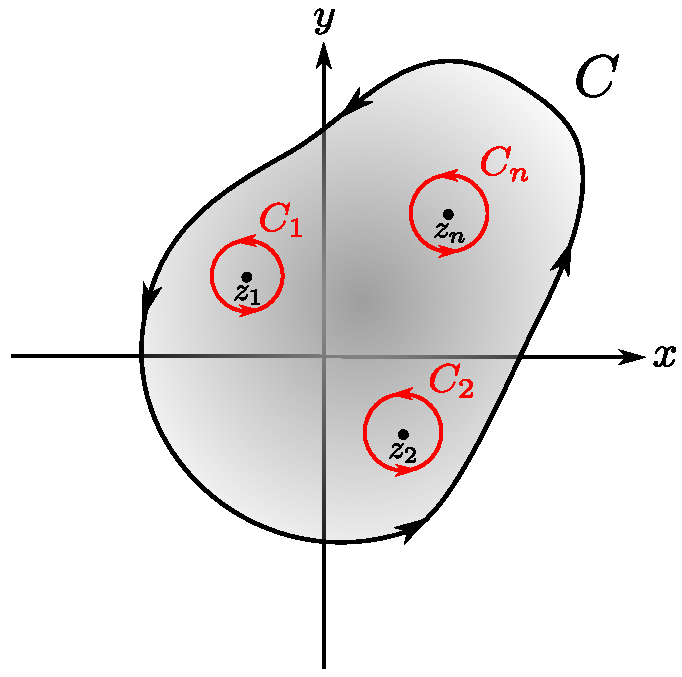
\includegraphics[scale = 0.55]{Figuras/TeoremaResiduo.pdf}
    \caption{Demostración teorema del residuo.}
    \label{fig:TeoResiduo}
\end{figure}
\end{proof}

\begin{ejemplo}
Evaluar la integral
$$\int_C \frac{5z-2}{z(z-1)} \,dz,$$

donde $C: |z| = 2$ está orientado positivamente.
\\

\textbf{Solución:} Notemos que $f(z) = \frac{5z-2}{z(z-1)}$ tiene puntos singulares aislados en $z = 0$ y $z = 1$, los cuales están en el interior de $C$. Debemos hallar los residuos de $f$ en $z = 0$ y $z = 1$, para ello usaremos la serie de Maclaurin
$$\frac{1}{1-z} = \sum_{n=0}^{\infty} z^n, \quad |z| < 1.$$

En primer lugar, escribimos el desarrollo de Laurent de $f$ en $0 < |z| < 1$:
\begin{align*}
 \frac{5z-2}{z(z-1)} = - \left( 5 - \frac{2}{z}\right) \frac{1}{1-z} &= - \left( 5 - \frac{2}{z}\right)  \sum_{n=0}^{\infty} z^n \\
 &= \sum_{n=0}^{\infty} 2z^{n-1} - \sum_{n=0}^{\infty} 5 z^n \\
 &= \frac{2}{z} - 3 - 3z - 3z^2 - \cdots 
\end{align*}

De aquí, $Res(f,0) = 2$. Por otro lado, para $0 < |z-1| < 1$, tenemos 
\begin{align*}
    \frac{5z-2}{z(z-1)} = \frac{5z-2}{z-1} \frac{1}{z} &= \frac{5z-2}{z-1} \frac{1}{1 + (z-1)} \\
    &= \frac{5z-5-2+5}{z-1} \sum_{n=0}^{\infty} (-1)^n (z-1)^n \\
    &= \left(5 + \frac{3}{z-1} \right) \sum_{n=0}^{\infty} (-1)^n (z-1)^n \\
    &=  \sum_{n=0}^{\infty} (-1)^n 5 (z-1)^n +  \sum_{n=0}^{\infty} (-1)^n 3 (z-1)^{n-1} \\
    &= \frac{3}{z-1} +2 -2(z-1) + 2(z-1)^2 - \cdots
\end{align*}

Así, $Res(f,1) = 3$. Por lo tanto,
$$\int_C \frac{5z-2}{z(z-1)} \,dz = 2\pi i\left[ Res(f,0) + Res(f,1)\right] = 10 \pi i.$$

\end{ejemplo}

\section{Ceros y polos}

\begin{defi}
Sea $f$ una función con un punto singular aislado $z_0$ y sea
$$f(z) = \sum_{n=0}^{\infty} a_n(z-z_0)^n + \sum_{n=1}^{\infty} \frac{b_n}{(z-z_0)^n}$$

su representación en serie de Laurent en un dominio $0 < |z-z_0| < R$.

\begin{enumerate}
    \item Llamaremos a:
    $$ \sum_{n=1}^{\infty} \frac{b_n}{(z-z_0)^n}$$
    
    \textbf{parte principal de $f$ en $z_0$}.
    
    \item Llamaremos a $z_0$ un \textbf{polo de orden $m$} si $b_m \neq 0$ y $b_{m+1} = b_{m+2} = \cdots = 0$. La serie de Laurent de $f$ en $z_0$ queda como sigue
    $$f(z) =  \sum_{n=0}^{\infty} a_n(z-z_0)^n +  \frac{b_1}{z-z_0} + \frac{b_2}{(z-z_0)^2} + \cdots + \frac{b_m}{(z-z_0)^m}, \quad 0 < |z-z_0| < R.$$
    
    \item Llamaremos \textbf{polo simple} si $z_0$ es un polo de orden 1.
    
    \item Llamaremos \textbf{punto singular esencial} si $b_m \neq 0$ para una infinidad de $m \in \mathbb{N}$.
    
    \item Diremos que $f$ tiene una \textbf{singularidad removible en $z_0$} si $f$ puede ser definida en $z_0$ de tal manera que sea analítica en $z_0$.
\end{enumerate}
\end{defi}

\begin{ejemplo}
La función 
$$f(z) = \frac{z^2-2z+3}{z-2}$$

tiene un polo simple en $z_0 = 2$. En efecto, si dividimos los polinomios:
\begin{figure}[H]
    \centering
    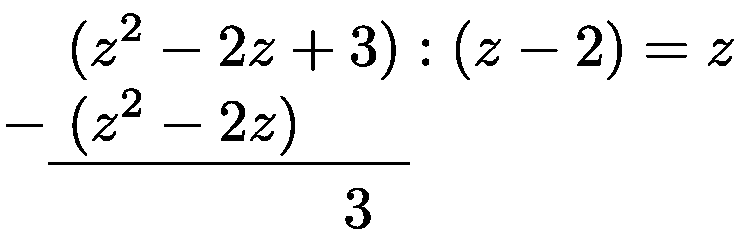
\includegraphics[scale = 0.4]{Figuras/DivisionPol.pdf}
\end{figure}

obtenemos que
$$\frac{z^2-2z+3}{z-2} = \frac{z(z-2) + 3}{z-2} = z + \frac{3}{z-2} =  (z-2) + 2 + \frac{3}{z-2}.$$
\end{ejemplo}

\begin{ejemplo}
Muestre que la función
$$f(z) = \frac{\sinh z}{z^4}$$

tiene un polo de orden $m = 3$ en $z_0 = 0$.
\\

\textbf{Solución:} Primero, determinemos la serie de Maclaurin de $\sinh z$. 

\begin{align*}
    \sinh z = \frac{e^z - e^{-z}}{2} &= \frac{1}{2} \left\{ \sum_{n=0}^{\infty} \frac{z^n}{n!} - \sum_{n=0}^{\infty} \frac{(-1)^n z^n}{n!}  \right\} \\
    &= \frac{1}{2} \sum_{n=0}^{\infty} \frac{(1-(-1)^n)}{n!} z^n \\
    &= \frac{1}{2} \sum_{k=0}^{\infty} \frac{(1-(-1)^{2k+1})}{(2k+1)!} z^{2k+1} \quad (n = 2k+1)\\
    &= \sum_{k=0}^{\infty} \frac{z^{2k+1}}{(2k+1)!}, \quad z \in \mathbb{C}.
\end{align*}

Luego,
\begin{align*}
 \frac{\sinh z}{z^4} = \sum_{k=0}^{\infty} \frac{z^{2k-3}}{(2k+1)!}& = \frac{1}{z^3} + \frac{1}{3!} \frac{1}{z} +\sum_{k=2}^{\infty} \frac{z^{2k-3}}{(2k+1)!} \\
 &=  \frac{1}{z^3} + \frac{1}{3!} \frac{1}{z} +\sum_{n=0}^{\infty} \frac{z^{2n+1}}{(2n+5)!}, \quad |z| > 0.    
\end{align*}

Claramente tiene un polo de orden 3 en $z_0 = 0$.

\end{ejemplo}

\begin{ejemplo}
La función
$$f(z) = e^{1/z} = \sum_{n=0}^{\infty} \frac{1}{n!} \frac{1}{z^n} = 1 +  \sum_{n=1}^{\infty} \frac{1}{n!} \frac{1}{z^n}, \quad |z| > 0$$

tiene un punto singular esencial en $z_0 = 0$.
\end{ejemplo}

\begin{ejemplo}
Considere la función 
$$f(z) = \frac{\sin z}{z}.$$

Sabemos que
$$\sin z = \sum_{n=0}^{\infty} \frac{(-1)^n}{(2n+1)!} z^{2n+1},$$

luego
\begin{align*}
    f(z) = \frac{\sin z}{z} &= \frac{1}{z}  \sum_{n=0}^{\infty} \frac{(-1)^n}{(2n+1)!} z^{2n+1} \\
    &= \sum_{n=0}^{\infty} \frac{(-1)^n}{(2n+1)!} z^{2n} = 1 - \frac{z^2}{3!} + \frac{z^4}{5!} - \cdots.
\end{align*}

Entonces, definiendo $f(0) = 1$, se tiene que $f$ es entera y la singularidad $z_0 = 0$ es removible. 
\end{ejemplo}

En general, si la serie de Laurent contiene sólo potencias no negativas de $z-z_0$, y la serie es, de hecho, una serie de potencias, $z_0$ es una singularidad removible. Si definimos $f$ en $z_0$ como $a_0$, la función pasa a ser analítica en $z_0$.

\begin{propo}
Sea $f$ una función analítica en una región $D$ con una singularidad aislada en $z_0$. Entonces, son equivalentes:
\begin{enumerate}
    \item $z_0$ es una singularidad removible.
    
    \item $f$ es acotada en $0 < |z-z_0| < R$.  
    
    \item $\lim\limits_{z\to z_0} f(z)$ existe.
    
    \item $\lim\limits_{z\to z_0} (z-z_0) f(z) = 0$.
\end{enumerate}
\end{propo}

\begin{proof}
\ 

\begin{itemize}
    \item  $(1) \Rightarrow (2), (3), (4)$: Supongamos que $z_0$ es una singularidad removible, se tiene que
    $$f(z) = \sum_{n=0}^{\infty} a_n (z-z_0)^n, \quad 0 < |z-z_0| < R.$$
    
    Luego, definiendo $f(z_0) = a_0$, $f$ es una función analítica en $D$. Por lo tanto, se sigue de manera inmediata (2), (3) y (4).
    
    \item $(2) \Rightarrow (4)$: Para  $0 < |z-z_0| < R$, tenemos que existe $M > 0$ tal que $|f(z)| \leq M $. Luego,
    $$|(z-z_0) f(z)| = |z-z_0| \,|f(z)| \leq M |z-z_0|.$$
    
    Por el teorema del acotamiento, cuando $z \to z_0$, tenemos que $\lim\limits_{z\to z_0} (z-z_0) f(z) = 0$.
    
    \item $(3) \Rightarrow (4)$: Por el álgebra de límites,
    $$\lim_{z\to z_0} (z-z_0) f(z) = \left( \lim_{z\to z_0} (z-z_0)  \right) \cdot \left(\lim_{z\to z_0} f(z) \right) = 0.$$
    
    \item $(4) \Rightarrow (1)$: Debemos demostrar que los $b_n = 0, n \in \mathbb{N}$. Sea $\varepsilon > 0$, existe $\delta > 0$ tal que
    $$0 < |z-z_0| < \delta \Rightarrow |f(z)| \,|z-z_0| < \varepsilon.$$
        Elijamos $r > 0$ con $r < 1$ y $r < \delta$, luego
    $$|z-z_0| = r \Rightarrow |f(z)| < \frac{\varepsilon}{|z-z_0|} = \frac{\varepsilon}{r}.$$
    
    Así,
    \begin{align*}
        |b_n| = \left| \frac{1}{2\pi i} \int_{C_r} \frac{f(\xi)}{(\xi-z_0)^{-n+1}} \,d\xi\right| &\leq \frac{1}{2\pi} \int_{C_r} |f(\xi)| \,|\xi-z_0|^{n-1} |d\xi| \\
        &< \frac{1}{2\pi} \int_{C_r} \frac{\varepsilon}{r} r^{n-1} \,|d\xi| \\
        &= \frac{1}{2\pi}\frac{\varepsilon}{r} r^{n-1} \int_{C_r}  \,|d\xi| \\
        &=  \frac{1}{2\pi}\frac{\varepsilon}{r} r^{n-1} 2\pi r \\
        &= \frac{\varepsilon}{r}r^n \leq \varepsilon.
    \end{align*}

Como $\varepsilon > 0$ es arbitrario, se concluye que, en el desarrollo de Laurent de $f$ en $z_0$, los $b_n = 0, n\in \mathbb{N}$.
\end{itemize}
\end{proof}

\begin{defi}
Sea $f$ analítica en una región $D$. Diremos que $f$ tiene un \textbf{cero de orden $m$ en $z_0$} si $f^{(i)}(z_0) = 0, i = 0,1,2, \dots, m-1$, y $f^{(m)}(z_0) \neq 0$.
\end{defi}

\begin{teorema} \label{TeoCerOrdenm}
Sea $f$ una función analítica en $z_0$. Entonces, $f$ tiene un cero de orden $m$ en $z_0$ si y sólo si $f(z)$ puede ser escrita como
\begin{equation}
 f(z) = (z-z_0)^m g(z),   \label{CerosOrdenm}
\end{equation}

donde $g$ es analítica en $z_0$ y $g(z_0) \neq 0$.
\end{teorema}

\begin{proof}
Dado que $f$ es analítica en $z_0$, entonces puede ser expandida en una serie de Taylor, es decir,
$$f(z) = \sum_{n=0}^{\infty} \frac{f^{(n)}(z_0)}{n!} (z-z_0)^n$$

en algún disco $B(z_0,R)$. Si $f$ tiene un cero de orden $m$ en $z_0$, entonces $f^{(i)}(z_0) = 0, i = 0,1,2, \dots, m-1$, y $f^{(m)}(z_0) \neq 0$. Por lo tanto, la serie de Taylor se reduce a 
$$f(z) = \sum_{n=m}^{\infty} \frac{f^{(n)}(z_0)}{n!} (z-z_0)^n = (z-z_0)^m \sum_{n=m}^{\infty} \frac{f^{(n)}(z_0)}{n!} (z-z_0)^{n-m}.$$

Como las series de potencias convergentes representan siempre funciones analíticas, podemos escribir
$$f(z) = (z-z_0)^m g(z),$$

donde $g$ es analítica en $|z-z_0| < R$ y $g(z_0) \neq 0$.

Por otro lado, supongamos que $f(z) = (z-z_0)^m g(z)$. Como $g$ es analítica en $z_0$, tiene una expansión en serie de Taylor 
$$g(z) = \sum_{n=0}^{\infty} b_n (z-z_0)^n,$$

ya que $g(z_0) \neq 0$, se sigue que $b_0 \neq 0$. Por lo tanto,
$$f(z) =  (z-z_0)^m  \sum_{n=0}^{\infty} b_n (z-z_0)^n = \sum_{n=0}^{\infty} b_n (z-z_0)^{m+n},$$

lo cual implica que $f$ tiene un cero de orden $m$ en $z_0$.

\end{proof}

Un teorema similar se tiene para los polos de orden $m$.

\begin{teorema} \label{TeoPoloOrdenm}
Una función $f$ tiene un polo de orden $m$ en $z_0$ si y sólo si, en alguna vecindad, sin su centro, de $z_0$,
\begin{equation}
f(z) = \frac{\phi(z)}{(z-z_0)^m},    \label{PoloOrdenm}
\end{equation}

donde $\phi$ es analítica en $z_0$ y $\phi(z_0) \neq 0$
\end{teorema}

\begin{proof}
 Supongamos que $f$ tiene un polo de orden $m$ en $z_0$, entonces su representación en serie de Laurent está dada por
\begin{align*}
 f(z) &= \frac{b_m}{(z-z_0)^m} + \cdots + \frac{b_1}{z-z_0} + \sum_{n=0}^{\infty} a_n (z-z_0)^n \\
 &= \frac{1}{(z-z_0)^m} \left\{ b_m + b_{m-1} (z-z_0) + \cdots + b_1 (z-z_0)^{m-1} + \sum_{n=0}^{\infty} a_n (z-z_0)^{n+m} \right\},
\end{align*}

para alguna región anular $0 < |z-z_0| < R$ y $b_m \neq 0$. Como lo que está entre corchetes es una serie de potencias, podemos escribir
\begin{equation*}
f(z) = \frac{\phi(z)}{(z-z_0)^m}, 
\end{equation*}

donde $\phi$ es analítica en $z_0$ y $\phi(z_0) = b_m \neq 0$. 

Por otro lado, supongamos que $f(z) = \phi(z)/(z-z_0)^m$, donde  $\phi$ es analítica en $z_0$ y $\phi(z_0) \neq 0$, entonces, por el teorema de Taylor,
$$g(z) = \sum_{n=0}^{\infty} c_n (z-z_0)^n, \quad c_0 = \phi(z_0) \neq 0.$$

Así, la serie de Laurent de $f$ alrededor de $z_0$ es
$$f(z) = \frac{1}{(z-z_0)^m} \sum_{n=0}^{\infty} c_n (z-z_0)^n = \frac{c_0}{(z-z_0)^m} + \frac{c_1}{(z-z_0)^{m-1}} + \cdots .$$

Como $c_0 \neq 0$, $z_0$ es un polo de orden $m$ para $f$.

\end{proof}

Las ceros y polos de una función está relacionados mediante el siguiente teorema.

\begin{teorema} \label{CeroYPolos}
Si $f$ es analítica en una vecindad de $z_0$, entonces $f$ tiene un cero de orden $m$ en $z_0$ si, y sólo si, $1/f$ tiene un polo de orden $m$ en $z_0$.
\end{teorema}

\begin{proof}
Supongamos que $m$ tiene un cero de orden $m$ en $z_0$, probemos que $1/f$ tiene un polo de orden $m$ en $z_0$. 

Usando \eqref{CerosOrdenm}, podemos escribir $f(z) = (z-z_0)^m g(z)$, con $g$ analítica en $z_0$ y $g(z_0) \neq 0$, por tanto, $g(z) \neq 0$ en una vecindad de $z_0$. En efecto, como analiticidad implica continuidad, tenemos
$$\lim_{z\to z_0} g(z) = g(z_0).$$

Para $\varepsilon = \frac{1}{2} g(z_0)$, existe $\delta >0$ tal que
$$0 < |z-z_0| < \delta \Rightarrow |g(z) - g(z_0)| < \frac{1}{2} g(z_0) \Leftrightarrow \frac{1}{2} g(z_0) < g(z) < \frac{3}{2} g(z_0).$$

Luego, $h(z) = \frac{1}{g(z)}$ es analítica en tal vecindad, ésto es,
$$\frac{1}{g(z)} = \sum_{n=0}^{\infty} a_n (z-z_0)^n, \quad |z-z_0| < \delta.$$

Entonces,
\begin{align*}
  \frac{1}{f(z)} &= \frac{1}{(z-z_0)^m}  \sum_{n=0}^{\infty} a_n (z-z_0)^n \\
  &=   \sum_{n=0}^{\infty} a_n (z-z_0)^{n-m} \\
  &= \frac{a_0}{(z-z_0)^{m}} + \frac{a_1}{(z - z_0)^{m-1}} + \cdots + \frac{a_{m-1}}{z-z_0} +  \sum_{n=m}^{\infty} a_n (z-z_0)^{n-m} \\
  &=  \frac{a_0}{(z-z_0)^{m}} + \frac{a_1}{(z - z_0)^{m-1}} + \cdots + \frac{a_{m-1}}{z-z_0} +  \sum_{n=0}^{\infty} a_{n+m} (z-z_0)^{n}.
\end{align*}

Por lo tanto, $\frac{1}{f(z)}$ tiene un polo de orden $m$.

Por otro lado, supongamos que $1/f$ tiene un polo de orden $m$ en $z_0$, usando \eqref{PoloOrdenm}, podemos escribir
\begin{equation*}
\frac{1}{f(z)} = \frac{\phi(z)}{(z-z_0)^m}, 
\end{equation*}

donde $\phi$ es analítica en $z_0$ y $\phi(z_0) \neq 0$, por tanto, $\phi(z) \neq 0$ en una vecindad de $z_0$. Luego, $\frac{1}{\phi(z)}$ es analítica en tal vecindad, ésto es,
$$\frac{1}{\phi(z)} = \sum_{n=0}^{\infty} c_n(z-z_0)^n, \quad |z-z_0| < \delta^*.$$

Entonces,
$$  f(z) = (z-z_0)^m  \sum_{n=0}^{\infty} c_n(z-z_0)^n =   \sum_{n=0}^{\infty} c_n (z-z_0)^{n+m}= \sum_{n=m}^{\infty} c_{n-m} (z-z_0)^n.$$

Lo que implica, por el teorema de Taylor, que
$$f^{(n)}(z_0) \neq 0, \quad n \geq m~~\mbox{y}~~ f^{(n)}(z_0) = 0, \quad n < m,$$

es decir, $f$ tiene un cero de orden $m$ en $z_0 = 0$.
\end{proof}

\section{Cálculo de residuos}

Hasta hora hemos determinado los residuos de una función encontrando su serie de Laurent, pero ésto no es necesario como lo veremos a continuación. 

\begin{teorema}
Sea $f$ una función analítica en una región $D$ con una singularidad aislada en $z_0$. Son equivalentes:
\begin{enumerate}
    \item $z_0$ es polo simple de $f$.
    
    \item $\lim\limits_{z\to z_0} (z-z_0) f(z) = b_1 \neq 0$.
\end{enumerate}
\end{teorema}

\begin{proof}
$z_0$ es un polo simple si y sólo si la serie de Laurent en $z_0$ tiene la forma
$$f(z) = \frac{b_1}{z-z_0} + a_0 + a_1 (z-z_0) + a_2(z-z_0)^2 + \cdots = \frac{b_1}{z-z_0} + g(z),$$

donde $b_1 \neq 0$ y $g$ es la serie de potencia analítica parte de la serie de Laurent. Entonces,
\begin{align*}
 (z-z_0)f(z) = b_1 + (z-z_0)g(z) \Leftrightarrow \lim_{z\to z_0} (z-z_0) f(z) &= b_1 + \left( \lim_{z\to z_0} (z-z_0)\right) \left(\lim_{z\to z_0} g(z) \right) \\
 &= b_1 + 0 a_0 = b_1.   
\end{align*}

\end{proof}

\begin{ejemplo}
Sea $C$ una curva simple cerrada orientada positivamente tal que $1$, $-i$ e $i$ están en su exterior y $-1$ en su exterior. Evaluar
$$\int_C \frac{1}{z^4+1} \,dz.$$

\textbf{Solución:} Notemos que
$$f(z) = \frac{1}{z^4+1} = \frac{1}{(z-1)(z+1)(z+i)(z-i)}.$$

Luego, la función $f$ tiene singularidades aisladas en $z = \pm 1, \pm i$. Tres de estas están en el interior de $C$, entonces, por el teorema del residuo,
$$\int_C \frac{1}{z^4+1} \,dz = 2\pi i \left[ Res(f,1) + Res(f,i) + Res(f,-i)\right].$$

Supongamos que tiene polos simples. Calculemos:
\begin{align*}
    \lim_{z\to 1} (z-1) \frac{1}{(z^4+1)}&= \lim_{z\to 1} \frac{1}{(z+1)(z-i)(z+i)} \\
    &= \left. \frac{1}{(z+1)(z-i)(z+i)} \right|_{z=1} \\
    &= \frac{1}{4}, \\
    \lim_{z\to i} (z-i) \frac{1}{(z^4+1)}&= \lim_{z\to i} \frac{1}{(z-1)(z+1)(z+i)} \\
    &= \left. \frac{1}{(z-1)(z+1)(z+i)} \right|_{z=i} \\
    &= \frac{i}{4} , \\
     \lim_{z\to -i} (z+i) \frac{1}{(z^4+1)}&= \lim_{z\to -i} \frac{1}{(z-1)(z+1)(z-i)} \\
    &= \left. \frac{1}{(z-1)(z+1)(z-i)} \right|_{z=-i} \\
    &= -\frac{i}{4}. 
\end{align*}

Como todos estos límites son distintos de cero, $z = 1,\pm i$ son polos simples de $f$ y
$$Res(f,1) = \frac{1}{4},~ Res(f,i) = \frac{i}{4}, ~ Res(f,-i) = - \frac{i}{4}.$$

Por lo tanto,
$$\int_C \frac{1}{z^4+1} \,dz = 2\pi i \left[ \frac{1}{4} + \frac{i}{4} - \frac{i}{4}\right] = \frac{\pi i}{2}.$$
\end{ejemplo}

Para polos de orden mayor, se tiene el siguiente teorema.

\begin{teorema}
Supongamos que $z_0$ es un polo de orden $m \geq 1$ de $f$. Entonces,
$$Re(f,z_0) = \lim_{z\to z_0} \frac{1}{(m-1)!} \frac{d^{m-1}}{dz^{m-1}}[(z-z_0)^m f(z)].$$
\end{teorema}

\begin{proof}
Como $z_0$ es un polo de orden $m\geq 1$ de $f$, entonces su serie de Laurent en $z_0$ tiene la forma
$$f(z) = \frac{b_m}{(z-z_0)^m} + \cdots + \frac{b_1}{z-z_0} + \sum_{n=0}^{\infty} a_n (z-z_0)^n.$$

Multiplicando por $(z-z_0)^m$, luego derivando $(m-1)$ veces, obtenemos
$$\frac{d^{m-1}}{dz^{m-1}}[(z-z_0)^m f(z)] = (m-1)! b_1 + \sum_{n=0}^{\infty} \frac{(n+m)!}{(n+1)!} a_n (z-z_0)^{n+1}.$$

Tomando el límite cuando $z\to z_0$, tenemos
$$\lim_{z\to z_0}  \frac{d^{m-1}}{dz^{m-1}}[(z-z_0)^m f(z)] = (m-1)! b_1 + 0.$$

Lo que implica que
$$\lim_{z\to z_0} \frac{1}{(m-1)!} \frac{d^{m-1}}{dz^{m-1}}[(z-z_0)^m f(z)] = b_1.$$
\end{proof}


\begin{ejemplo}
Determine el residuo de 
$$f(z) = \frac{z^2}{(z^2+\pi^2)^2 \sin z}$$

en $z_0 = i\pi$.
\\

\textbf{Solución:} La función $f$ es analítica excepto cuando $z^2 + \pi^2 = 0$ o $\sin z = 0$. Por lo tanto, $f$ tiene singularidades aisladas en $\pm i \pi$ y en $k\pi$ con $k \in \mathbb{Z}$. Para determinar el residuo de $f$ en $z_0 = i\pi$, consideremos la función
$$\frac{1}{f(z)} = \frac{(z+i\pi)^2 (z-i\pi)^2 \sin z}{z^2} = (z-i\pi)^2 \frac{(z+i\pi)^2 \sin z}{z^2},$$

la cual tiene la forma
$$(z-i\pi)^2 g(z)$$

con $g$ analítica en $z_0= i\pi $ y $g(z_0) \neq i\pi$. Luego, $1/f$ tiene un cero de orden 2 en $i\pi$. Entonces, por el teorema \ref{CeroYPolos}, $f$ tiene un polo de orden $2$. Así,
\begin{align*}
    Res(f,i\pi) &= \lim_{z\to i\pi} \frac{d}{dz} [(z-i\pi)^2 f(z)] \\
    &= \lim_{z\to i\pi} \frac{d}{dz} \left[\frac{z^2}{(z+i\pi)^2 \sin z}\right]  \\
    &= \lim_{z\to i\pi} \frac{2z(z+i\pi)\sin z - z^2 ((z+i\pi) \cos z + 2\sin z)}{(z+i\pi)^3 \sin^2(z)} \\
    &= \frac{2\sinh(\pi) + (-\pi \cosh(\pi) - \sinh(z))}{-4\pi \sinh^2(\pi)} = - \frac{1}{4\pi \sinh(\pi)} + \frac{\cosh(\pi)}{4\pi \sinh^2(\pi)}.
\end{align*}

\end{ejemplo}

\begin{propo}
Sean $g$ y $h$ analíticas en $z_0$ y suponga que $g(z_0) \neq 0$, $h(z_0) = 0$ y $h'(z_0) \neq 0$. Entonces, $f(z) = g(z)/h(z)$ tiene un polo simple en $z_0$, y
$$Res(f,z_0) = \frac{g(z_0)}{h'(z_0)}.$$
\end{propo}

\begin{proof}
Sabemos que
$$\lim_{z\to z_0} \frac{h(z) - h(z_0)}{z-z_0} = \lim_{z\to z_0} \frac{h(z)}{z-z_0} = h'(z_0) \neq 0.$$

Entonces,
$$\lim_{z\to z_0} \frac{z-z_0}{h(z)} = \frac{1}{h'(z_0)}.$$

Así,
$$\lim_{z\to z_0} (z-z_0) f(z) = \lim_{z\to z_0} (z-z_0) \frac{g(z)}{h(z)} = \frac{g(z_0)}{h'(z_0)}$$

existe y es distinto de cero. Por lo tanto, $f$ tiene un polo simple y 
$$Res(f,z_0) = \frac{g(z_0)}{h'(z_0)}.$$
\end{proof}

\section{Integrales reales impropias}

En esta sección se entregará una técnica útil para evaluar integrales impropias del tipo
$$\int_{-\infty}^b f(x) \,dx ~~\mbox{y}~~ \int_a^{\infty} f(x) \,dx, \quad a,b \in \mathbb{R},$$

donde $f$ es continua en todo intervalo cerrado dentro del intervalo de integración. Además, de
$$\int_{-\infty}^{\infty} f(x)\,dx$$

donde $f$ es continua en $\mathbb{R}$.

Sabemos del cálculo integral de una variable que $\int_{-\infty}^{\infty} f(x)\,dx$ converge si
$$\lim_{a \to - \infty} \int_{a}^{0}f(x) \,dx; \quad \lim_{b \to + \infty} \int_{0}^{b}f(x) \,dx$$

existen y, en tal caso,
$$\int_{-\infty}^{\infty} f(x) \,x = \lim_{a \to - \infty} \int_{a}^{0}f(x) \,dx +  \lim_{b \to + \infty} \int_{0}^{b}f(x) \,dx .$$

\begin{defi}
Definimos el \textbf{valor principal de Cauchy} de la integral $\int_{-\infty}^{\infty} f(x)\,dx$ a
$$V.P. \int_{- \infty}^{\infty} f(x) \,dx = \lim_{a\to + \infty} \int_{-a}^a f(x)\,dx$$

si el límite existe.
\end{defi}

\textbf{Observación:} El valor principal de Cauchy de una integral puede existir incluso cuando la integral en si misma no es convergente. Por ejemplo, $\int_{-a}^ax dx = 0$ para todo $a$, lo cual implica que $V.P. \int_{-\infty}^{\infty} xdx = 0$, pero la integral en si no converge, pues $\int_0^{\infty} xdx = \infty$. Sin embargo, 
$$\int_{\infty}^{\infty} f(x) \,dx < \infty \Rightarrow V.P. \int_{\infty}^{\infty} f(x) \,dx < \infty$$

y ambas integrales coinciden. En efecto, los límites
$$\lim_{a \to \infty} \int_{-a}^{0}f(x) \,dx; \quad \lim_{a \to + \infty} \int_{0}^{a}f(x) \,dx$$

existen y
\begin{align*}
   V.P. \int_{- \infty}^{\infty} f(x) \,dx &= \lim_{a\to + \infty} \int_{-a}^a f(x)\,dx  \\
   &= \lim_{a\to + \infty} \left(\int_{-a}^{0} f(x) \,dx + \int_0^a f(x) \,dx \right) \\
   &= \lim_{a\to + \infty} \int_{-a}^{0} f(x) \,dx +  \lim_{a\to + \infty}\int_0^a f(x) \,dx \\
   &= \int_{- \infty}^{+\infty} f(x) \,dx.
\end{align*} 

Pero supongamos que $f$ es una función par, es decir, $f(-x) = f(x)$ para todo $x \in \mathbb{R}$. Entonces, si el valor principal de Cauchy existe, la integral converge al mismo valor (demuéstrelo!!!!!). De hecho,
\begin{equation}
 \int_0^{+\infty} f(x) \,dx = \frac{1}{2} \int_{-\infty}^{+ \infty} f(x) \,dx. \label{IntIPar}   
\end{equation}

Nuestro propósito será calcular el V.P. Para ilustrar el método, analicemos el siguiente ejemplo.

\begin{ejemplo} \label{EjImpropia1}
Calcular 
$$\int_0^{\infty} \frac{2x^2-1}{x^4+5x^2+4} \,dx.$$

\textbf{Solución:} La función
$$f(x) =  \frac{2x^2-1}{x^4+5x^2+4}$$

es continua en $\mathbb{R}$ y es una función par. Luego,
$$\int_0^{\infty} \frac{2x^2-1}{x^4+5x^2+4} \,dx = \frac{1}{2} \int_{-\infty}^{\infty} \frac{2x^2-1}{x^4+5x^2+4} \,dx.$$

Extendamos la función $f$ a todo $\mathbb{C}$, 
$$f(z) = \frac{2z^2-1}{z^4+5z^2+4} = \frac{2z^2-1}{(z^2+1)(z^2+4)},$$

excepto para los puntos donde $z^4+5z^2+4 = 0$; $\pm i, \pm 2 i$. Consideremos la curva simple cerrada suave por tramos $\gamma = C_R + S_{-R,R}$ orientada positivamente, donde $R > 2$ (para que las singularidades estén dentro de $\gamma$), $C_R$ es la semicircunferencia $|z| = R$ y $S_{-R,R}$ es el segmento dirigido de $-R$ a $R$ (ver figura \ref{fig:IntegralImpropia1}).

\begin{figure}[H]
    \centering
    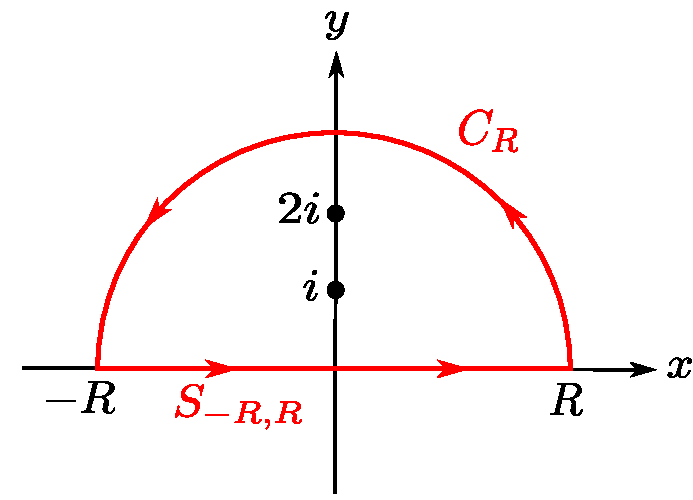
\includegraphics[scale = 0.6]{Figuras/IntegralImpropia1.pdf}
    \caption{La curva de integración para el ejemplo \ref{EjImpropia1}.}
    \label{fig:IntegralImpropia1}
\end{figure}

Por el teorema de residuos,
$$\int_{\gamma} f(z) \,dz = 2\pi i [Res(f,i) + Res(f,2i)].$$

Pero,
$$\int_{\gamma} f(z) \,dz = \int_{-R}^R f(x) \,dx + \int_{C_R}f(z)\,dz.$$

De acuerdo al cálculo de residuos,
\begin{align*}
    Res(f,i) &= \lim_{z\to i} (z-i)f(z) = \frac{i}{2}, \\
    Res(f,2i) &= \lim_{z\to 2i} (z-2i)f(z) = -\frac{3i}{4}.
\end{align*}

Por lo tanto,
$$\int_{-R}^R f(x) \,dx + \int_{C_R}f(z)\,dz = 2\pi i \left[\frac{i}{2} - \frac{3i}{4}\right] = \frac{\pi}{2}.$$

Lo que implica
$$\int_{-R}^R f(x) \,dx = \frac{\pi}{2} - \int_{C_R}f(z)\,dz.$$

Queda por analizar el comportamiento de $\int_{C_R} f(z) \,dz$. Para ello, notemos que para $|z| = R$:
$$|2z^2-1| \leq 2|z|^2 +1 = 2R^2+1$$

y
$$|z^4+5z^2+4| = |z^2+1|\,|z^2+4| \geq ||z|^2 - 1|\,||z|^2-4| = (R^2-1)(R^2-4).$$

Entonces, para cualquier $z \in C_R$,
$$\left| \frac{2z^2-1}{z^4+5z^2+4} \right| \leq \frac{2R^2+1}{(R^2-1)(R^2-4)}$$

y ésto significa que 
$$\left|\int_{C_R} f(z) \,dz \right| \leq\frac{2R^2+1}{(R^2-1)(R^2-4)} \pi R.$$

Como
$$\lim_{R \to + \infty} \frac{2R^2+1}{(R^2-1)(R^2-4)} \pi R = 0 \Rightarrow \lim_{R \to + \infty} \int_{C_R} f(z) \,dz = 0.$$

Así,
$$\lim_{R \to + \infty} \int_{-R}^R f(x) \,dx = \frac{\pi}{2} - \lim_{R\to + \infty} \int_{C_R} f(z) \,dz = \frac{\pi}{2},$$

o sea
$$V.P. \int_{-\infty}^{\infty}  \frac{2x^2-1}{x^4+5x^2+4} \,dx = \frac{\pi}{2}.$$

Como el integrando es par, sabemos que la integral converge a su valor principal de Cauchy, y de acuerdo con la ecuación \eqref{IntIPar},
$$\int_0^{\infty} \frac{2x^2-1}{x^4+5x^2+4} \,dx = \frac{1}{2}  \int_{-\infty}^{\infty}  \frac{2x^2-1}{x^4+5x^2+4} \,dx = \frac{\pi}{4}.$$

Se obtiene el mismo resultado al tomar la semicircunferencia por debajo del eje real ($Im(z) < 0$), pero para que coincidan los signos, la orientación debe ser negativa.
\end{ejemplo}

El procedimiento anterior funciona siempre y cuando se satisfagan las hipótesis del siguiente teorema.

\begin{teorema}
Sea $f$ una función analítica con un número finito de puntos singulares aislados $z_1, \dots, z_n$, todos ellos ubicados en la región $Im (z) > 0$. Entonces,
$$\lim_{R\to + \infty} \sup_{|z| \leq R} |zf(z)| = 0 \Rightarrow \lim_{R\to + \infty} \int_{-R}^R f(x) \,dx = 2\pi i \sum_{i=1}^n Res(f,z_i).$$
\end{teorema}

\begin{proof}
Sea $\gamma = C_R + S_{-R,R}$ una curva cerrada, suave a trazos orientada positivamente con $R > \max\{|z_i| : i = 1,2, \dots, n\}$, como en la figura,

\begin{figure}[H]
    \centering
    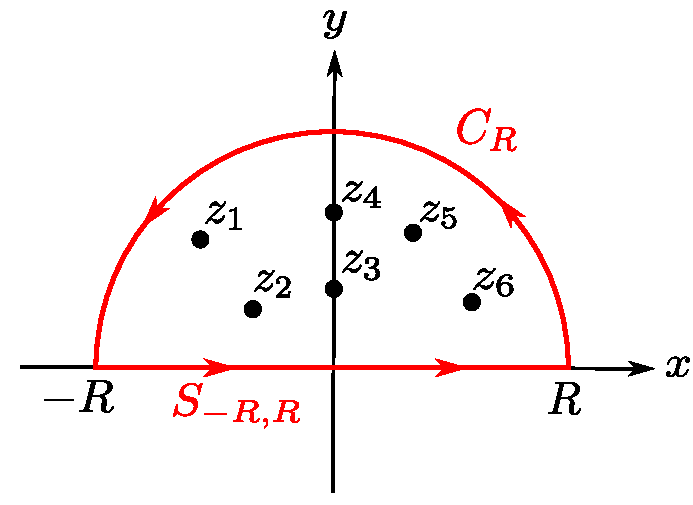
\includegraphics[scale = 0.6]{Figuras/IntegralImpropia2.pdf}
    \caption{La curva de integración para la demostración del teorema.}
    \label{fig:IntegralImpropia2}
\end{figure}

Por el teorema del residuo, tenemos que
$$\int_{\gamma} f(z)\,dz = 2\pi i \sum_{i=1}^n Res(f,z_i).$$

Ahora, 
\begin{align*}
    \int_{\gamma} f(z) \,dz &= \int_{-R}^R f(x) \,dx + \int_{C_R} f(z) \,dz \\
    \Rightarrow \int_{-R}^R f(x) \,dx &=  2\pi i \sum_{i=1}^n Res(f,z_i) - \int_{C_R} f(z) \,dz.
\end{align*}

Como $f$ es continua en $C_R$, $|f(z)|$ está acotada tal que
$$\forall z \in C_R: ~ |f(z)| \leq \sup_{z \in C_R} |f(z)| < \infty.$$

Luego,
$$\left| \int_{C_R} f(z) \,dz \right| \leq \pi R \sup_{z \in C_R} |f(z)|.$$

Por propiedades del supremo y teniendo en cuenta que estamos estudiando la integral para los $|z| = R$, se tiene que
$$R \sup_{z \in C_R} |f(z)| = \sup_{z \in C_R} R |f(z)| =\sup_{z \in C_R} |z f(z)|.$$

Entonces,
$$\left| \int_{C_R} f(z) \,dz \right| \leq \pi \sup_{z \in C_R} |zf(z)|.$$

Por hipótesis,
$$\lim_{R\to + \infty} \sup_{|z| \leq R} |zf(z)| = 0  \Rightarrow  \int_{C_R} f(z) \,dz  = 0.$$

Por lo tanto,
$$\lim_{R \to + \infty} \int_{-R}^R f(x) \,dx = 2\pi i \sum_{i=1}^n Res(f,z_i) - \lim_{R\to + \infty} \int_{C_R} f(z) \,dz = 2\pi i \sum_{i=1}^n Res(f,z_i).$$
\end{proof}

Ahora nos centraremos en calcular integrales impropias convergentes del tipo
$$\int_{-\infty}^{\infty} f(x) \sin(ax) \,dx ~~\mbox{y}~~ \int_{-\infty}^{\infty} f(x) \cos(ax) \,dx$$

donde $a$ denota una constante positiva. El método descrito anteriormente no es aplicable directamente, pues $\sin z$ y $\cos z$ crecen como $\sinh y$ o $e^{ay}$, al tender $y$ al infinito. La modificación se ilustra en el siguiente ejemplo.

\begin{ejemplo} \label{EjImpropia2}
Calcular la integral impropia
$$\int_{- \infty}^{\infty} \frac{\cos(x)}{1+x^2} dx.$$

\textbf{Solución:} La integral es convergente, pues
$$\forall x \in \mathbb{R}: ~\left| \frac{\cos(x)}{1+x^2} \right| \leq \frac{1}{1+x^2}$$

y
$$\int_{-\infty}^{\infty} \frac{1}{1+x^2} \,dx = \pi.$$

Para determinar su valor, consideremos la integral compleja
$$\int_{\gamma} \frac{e^{iz}}{1+z^2} \,dz,$$

donde $\gamma = C_R + S_{-R,R}$ orientada positivamente con $R > 1$ (ver figura \ref{fig:IntegralImpropia3}). El integrando tiene solo la singularidad aislada $z = i$ dentro de la curva de integración. Entonces, por el teorema del residuo,
$$\int_{\gamma} \frac{e^{iz}}{1+z^2} \,dz = \int_{-R}^R \frac{e^{ix}}{1+x^2} \,dx + \int_{C_R} \frac{e^{iz}}{1+z^2} \,dz = 2\pi i Res(f,i).$$

\begin{figure}[H]
    \centering
    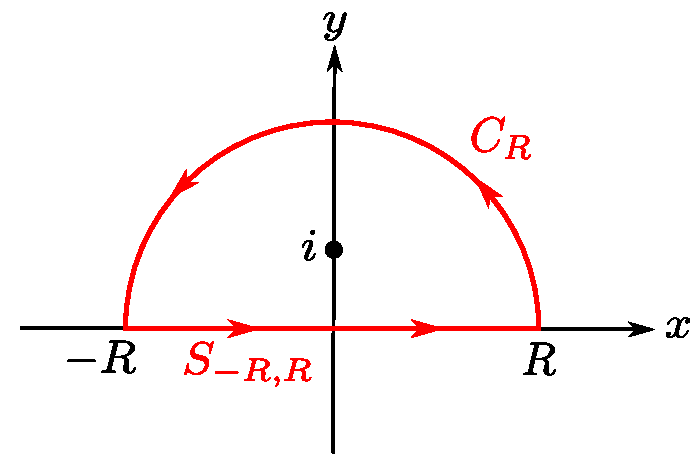
\includegraphics[scale = 0.6]{Figuras/IntegralImpropia3.pdf}
    \caption{La curva de integración para el ejemplo \ref{EjImpropia2}.}
    \label{fig:IntegralImpropia3}
\end{figure}

Ahora,
$$Res(f,i) = \lim_{z\to i} (z-i) \frac{e^{iz}}{1+z^2} = \lim_{z\to i} \frac{e^{iz}}{z+i} = - \frac{1}{2} i e^{-1}.$$

Así,
$$ \int_{-R}^R \frac{e^{ix}}{1+x^2} \,dx = \frac{\pi}{e} - \int_{C_R} \frac{e^{iz}}{1+z^2} \,dz.$$

Acotando el integrando sobre $C_R$:
$$\forall z \in C_R: ~ \left| \frac{e^{iz}}{1+z^2} \right| \leq \frac{1}{|1 - |z|^2|} = \frac{1}{R^2-1}.$$

Luego,
$$\left|\int_{C_R} \frac{e^{iz}}{1+z^2}\right| \leq \frac{1}{R^2-1} \pi R.$$

Como
$$\lim_{R\to + \infty} \frac{\pi R}{R^2-1} = 0 \Rightarrow \lim_{R\to + \infty} \int_{C_R} \frac{e^{iz}}{1+z^2} = 0.$$

Por lo tanto,
$$\lim_{R \to + \infty} \int_{-R}^R \frac{e^{ix}}{1+x^2} \,dx = \frac{\pi}{e} - \lim_{R\to + \infty} \int_{C_R} f(z) \,dz =  \frac{\pi}{e}.$$

Pero,
$$\int_{-R}^R \frac{e^{ix}}{1+x^2} \,dx = \int_{-R}^R \frac{\cos(x)}{1+x^2} \,dx + i \int_{-R}^R \frac{\sin x}{1+x^2} \,dx.$$

Como
$$\int_{-R}^R \frac{\sin(x)}{1+x^2} \,dx = 0 \quad  \mbox{(Integrando impar)},$$

tenemos que
$$\lim_{R \to + \infty} \int_{-R}^R \frac{e^{ix}}{1+x^2} \,dx = \lim_{R \to + \infty} \int_{-R}^R \frac{\cos(x)}{1+x^2} \,dx = \frac{\pi}{e}.$$

Como el integrando es par,
$$\int_{-\infty}^{\infty}\frac{\cos(x)}{1+x^2} \,dx = \frac{\pi}{e}. $$

\end{ejemplo}

\begin{lema}[Lema de Jordan]
La siguiente desigualdad es válida para $a > 0$:
$$\int_{0}^{\pi} e^{-a \sin \theta} d\theta \leq \frac{\pi}{a}.$$
\end{lema}

\begin{proof}
Comenzamos escribiendo
$$\int_0^{\pi} e^{-a \sin \theta} d\theta = \int_0^{\pi/2} e^{-a \sin \theta} d\theta + \int_{\pi/2}^{\pi} e^{-a \sin \theta} d\theta.$$

Haciendo el cambio de variable $u = \pi - \theta \Rightarrow du = -d\theta$ en la segunda integral y notando que $\sin (\theta) = \sin(\pi - u) =  \sin(u)$, obtenemos
\begin{equation}
\int_0^{\pi} e^{-a \sin \theta} d\theta = \int_0^{\pi/2} e^{-a \sin \theta} d\theta - \int_{\pi/2}^{0} e^{-a \sin u} d u = 2 \int_0^{\pi/2} e^{-a \sin \theta} d\theta.    \label{Jordan1}
\end{equation}

Probemos la desigualdad de Jordan:
\begin{equation}
\forall \theta \in [0, \pi/2]:~ \sin \theta \geq \frac{2}{\pi} \theta.    \label{DesiJordan}
\end{equation}

Para ello, consideremos la integral
$$\int_0^1 \left[\cos(\theta x) - \cos\left( \frac{\pi x }{2}\right)\right]\,dx, \quad  \theta \in ]0,2\pi[.$$

la cual representa el área entre las curvas $\cos(\theta x)$ y $\cos\left( \frac{\pi x}{2}\right)$ en $[0,1]$. Como este integral es positiva,
$$\int_0^1 \left[\cos(\theta x) - \cos\left( \frac{\pi x }{2}\right)\right] = \frac{\sin \theta}{\theta} - \frac{2}{\pi} \geq 0 \Rightarrow \sin \theta \geq \frac{2\theta}{\pi} .$$

La desigualdad \eqref{DesiJordan} implica que $-a \sin \theta \leq - \frac{2}{\pi} a \theta$ y combinado esto con \eqref{Jordan1}, deducimos que
$$\int_{0}^{\pi} e^{-a \sin \theta} \,d \theta \leq 2 \int_{0}^{\pi/2} e^{- \frac{2}{\pi} a \theta} \,d\theta = \left. - \frac{\pi}{a} e^{-\frac{2}{\pi} a\theta}\right|_{0}^{\pi/2} = \frac{\pi}{a}(1-e^{-a}) \leq \frac{\pi}{a}.$$
\end{proof}

\begin{teorema}
Sea $f$ una función analítica con un número finito de puntos singulares aislados $z_1, \dots, z_n$, todos ellos ubicados en la región $Im(z) > 0$. Entonces,
$$\lim_{R\to + \infty} \sup_{|z| \leq R} |f(z)| = 0 \Rightarrow \lim_{R\to + \infty} \int_{-R}^R f(x) e^{i\alpha x}\,dx = 2\pi i \sum_{i=1}^n Res(f(z) e^{i\alpha z},z_i), \quad \alpha > 0.$$
\end{teorema}

\begin{proof}
Sea $\gamma = C_R + S_{-R,R}$ una curva cerrada, suave a trazos orientada positivamente con $R > \max\{|z_i| : i = 1,2, \dots, n\}$, como en la figura,

\begin{figure}[H]
    \centering
    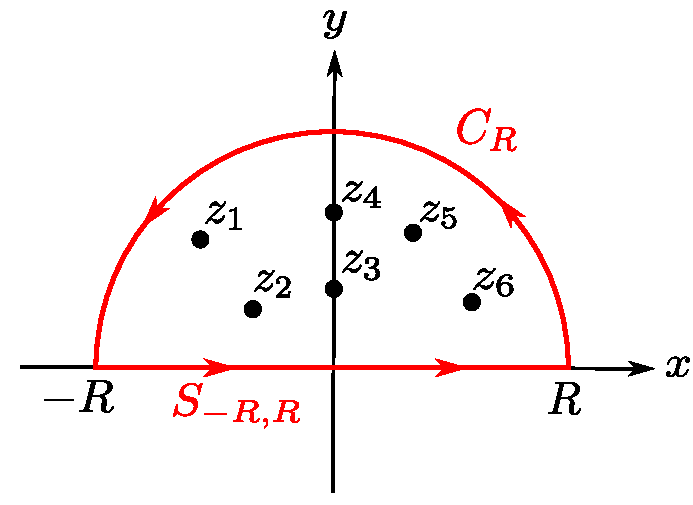
\includegraphics[scale = 0.6]{Figuras/IntegralImpropia2.pdf}
    \caption{La curva de integración para la demostración del teorema.}
    \label{fig:IntegralImpropia6}
\end{figure}

Por el teorema del residuo, tenemos que
$$\int_{\gamma} f(z) e^{i\alpha z}\,dz = 2\pi i \sum_{i=1}^n Res(f(z) e^{i\alpha z},z_i).$$

Ahora, 
\begin{align*}
    \int_{\gamma} f(z) e^{i\alpha z} \,dz &= \int_{-R}^R f(x) e^{i\alpha x} \,dx + \int_{C_R} f(z)  e^{i\alpha z} \,dz \\
    \Rightarrow \int_{-R}^R f(x) e^{i\alpha x}\,dx &=  2\pi i \sum_{i=1}^n Res(f(z) e^{i\alpha z},z_i) - \int_{C_R} f(z)  e^{i\alpha z} \,dz.
\end{align*}

Como $f$ es continua en $C_R$, $|f(z)|$ está acotada tal que
$$\forall z \in C_R: ~ |f(z)| \leq \sup_{z \in C_R} |f(z)| = M(R) < \infty.$$

Luego,
\begin{align*}
 \left| \int_{C_R} f(z) e^{i\alpha z} \,dz \right| &=  \left| \int_0^{\pi} f(R e^{i\theta}) e^{i \alpha R e^{i\theta}} i Re^{i\theta}d\theta \right| \\
 &\leq \int_0^{\pi}|f(R e^{i\theta})| \, \left|e^{i \alpha R (\cos \theta + i \sin \theta)} \right| \,|i Re^{i\theta}|\,d\theta \\
 &\leq \int_0^{\pi} M(R) e^{-\alpha R\sin\theta} R \,d\theta \\
 &= R M(R) \int_0^{\pi} e^{-\alpha R\sin\theta} \,d\theta \\
 &\leq R M(R) \frac{\pi}{\alpha R} = \frac{\pi}{\alpha} M(R).
\end{align*}

Por hipótesis,
$$\lim_{R\to + \infty} \sup_{|z| \leq R} |f(z)| = 0  \Rightarrow \lim_{R \to + \infty} \int_{C_R} f(z) e^{i\alpha z} \,dz   = 0.$$

Por lo tanto,
\begin{align*}
\lim_{R\to + \infty} \int_{-R}^R f(x) e^{i\alpha x}\,dx &= 2\pi i \sum_{i=1}^n Res(f(z) e^{i\alpha z},z_i) - \lim_{R\to + \infty} \int_{C_R} f(z) e^{i\alpha z} \,dz  \\
&= 2\pi i \sum_{i=1}^n Res(f(z) e^{i\alpha z},z_i).    
\end{align*}

\end{proof}

